%\newpage

\section{Key data structures}
\label{design}

In this section, we will examine the techniques for implementing
workshares in a parallel region. 

%The data structures is explained in a ``top-down'' manner.
 
\subsection{General requirement}
\label{sec:require}

The specific ways of implementing workshares in a parallel region may
be different from one to another, but with the analysis we already
have in previous sections, one can see that at least the following
data segments should be in a \emph{control block} for workshares,

\begin{itemize}
\item \emph{Structure to hold workshare-specific information} This is
  needed to store information regarding an OpenMP DO construct or
  SECTIONS construct. Things like initial, final value of the loop
  induction variable, the schedule type, etc.
\item \emph{Structure to complete possible barrier synchronization}
  This is used to implement any barriers that may be needed during the
  lifetime of the workshare construct.
\item \emph{Structure to control access to the workshare control
    block} This is typically a \emph{lock} to ensure only one thread
  modifies the information of the shared control block, for example,
  to mark the workshare started or show that a particular section code is
  already done.
\end{itemize}

Since different workshare constructs can be put into the same parallel
region, the first item must be a ``\emph{per workshare}'' value, i.e.
for each workshare in the parallel region, there should be a
corresponding one. Because of the existence of NOWAIT clauses,
multiple workshares can be \emph{active} at the same time --- executed
by different threads simultaneously.  So, multiple instance of this
data structure must exist simultaneously; one for each active
workshare. The same observation can be made for the third item in the
list. Each thread will access its own active workshare control block,
which may or may not be different from each other.

%Discussion on the second item is out of the interest in this note, for
%general structures to implement a barrier synchronization, please
%refer to \cite{Mel91}.

In general, there has to be a queue of workshare control blocks for
each parallel region.

\subsection{The control block queue length}
\label{sec:size}

Once we understand the basic structures needed for a parallel region,
we have to consider its construction, destruction and initialization.
At the same time, we need to minimize the overhead of creating and
manipulating such structures, as noted in \cite{Bul99}.

It cannot be statically predicted how many parallel regions a program
may explore and how many of them will be active at the same time because 
of nested parallelism or explicit usage of threads in user codes.
Therefore, the workshare control block queue will be allocated
dynamically. In addition to discussions in section \ref{sec:require}, a
workshare control block queue has to be constructed whenever a
parallel region is encountered, and it will be destroyed when the
parallel region ends.

Before we go any further, we need to decide the length of this queue.
For example, if we map each workshare to its own control block
in a straightforward manner, the following parallel region

{\small
\begin{verbatim}
      !$OMP PARALLEL 
      !$OMP DO
            DO i = istart, iend
              ...
            END DO
      !$OMP END DO
      !$OMP DO
            DO i = istart, iend
            ...
            END DO 
      !$OMP END DO NOWAIT
      !$OMP DO
            DO i = istart, iend
            ...
            END DO
      !$OMP END DO
      !$OMP DO
            DO i = istart, iend
            ...
            END DO
      !$OMP END DO
      !$OMP END PARALLEL
\end{verbatim}
}

will need the workshare control block queue as shown in Figure
\ref{fig:queue}, where there are four block elements in total.

\begin{figure}[!h]
  \begin{center}
    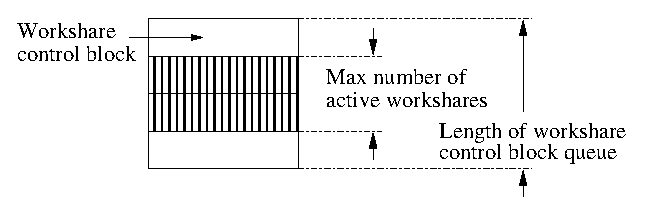
\includegraphics[angle=0, width=0.7\textwidth]{queue.eps}
    \caption{\footnotesize Workshare control block queue}
    \label{fig:queue}
  \end{center}
\end{figure}

A simple way of handling the queue is to create a new control block
whenever a workshare is encountered, more accurately, whenever a
\emph{workshare instance} is encountered. If a workshare is defined
inside a sequential loop body, we have as many workshare instances as
the number of iterations in that loop.

Since the workshare control block is a shared construct for multiple
threads, to constantly increase its size will be detrimental to the
runtime overhead for the creation of parallel regions. Moreover, doing so
will create higher memory impact on the overall program execution.

A better solution is to allocate a chunk of workshare control blocks
at once, use them as a block pool, and try to reuse the pool whenever 
possible, only increasing its size when absolutely necessary.

In the queue, we will set up extra fields, such as \emph{next
  available workshare control block pointer}, and set it back to the
beginning whenever an explicit or implicit barrier is met. Thus we
only need two block structures instead of the four in Figure
\ref{fig:queue} for the code snippet above. When the first workshare
instance finishes, a barrier synchronization occurs, and the next
available workshare control pointer will be set back to the first
block structure. Then, two block structures are needed at most because of
the NOWAIT clause. After that, another barrier will set the pointer
back to the beginning again.

%The length needed for the queue is actually the maximum number of
%active workshares in the parallel region. We can allocate a chunk of
%workshare control blocks as the initial pool, then with the method
%described above keep reusing it. This will also help to improve the
%cache locality of the program. 

Furthermore, resizing the pool may need extra book-keeping structures
and work. If we artificially introduce a barrier on a nowait workshare
when the queue becomes full, we do not need to increase the size at
all\footnote{We do need to mark the head and tail position of the
active workshares in the queue, so the next available pointer can be
set, from the position next to the head, back to its tail when a
barrier is encountered.}.

In real applications, a special case of using of NOWAIT clauses is to
form a coarse-grain software pipeline, such as the one in APPLU of
SPECOMP2001\cite{Spe01}, thus one cannot degrade any nowait
workshare. But in such cases, the length of the pipeline is often set
as the number of the hardware processors to get best performance.
Choosing a proper fixed-size queue to avoid extra overhead is still a
valid consideration.

Regardless of resizing the queue or not, the number of hardware
processors or its multiples, to be conservative, is a good candidate
for the initial chunk size of the pool. Then we can resize the queue
if needed.

\subsection{Fine-grained optimization}
\label{sec:optimize}

From the analysis in section \ref{sec:require}, a lock has to be defined
within the control block structure. Whether it is hand coded as in
\cite{Mel91} or used directly from Pthread library\cite{But97}, the
lock itself needs to be initialized, along with other structures for
the workshare-specific information.

The master thread can initialize all the structures at once when they
are allocated during the setup time. But for parallel regions where
the maximum number of active workshares is small --- only one, when
the NOWAIT clause does not exist, this process will bring extra overhead.
It is more desirable to defer the initialization of the block items
until their use becomes necessary.

Algorithm \ref{alg:workshare}, used to execute a workshare, achieved
this by always keeping the queue have one extra block ready during
initialization phase. In the scheme, the master thread initializes the
first control block, thus making the queue ready to use for the first
workshare. Then, when the first thread exclusively accesses the
available control block through the lock, it will make the next
control block available by initializing it.

%A counter may be used to indicate how many blocks have been
%initialized. 

\begin{algorithm}[h]
  \SetLine %this is vertical line
{\small
  \AlgData{Workshare control block queue}
%    allocated and with its first element initialized by the master thread}
  \AlgData{Next available block pointer}
  \BlankLine

  \Begin {
    \If{this workshare is not locked} {
      lock it\;
      \eIf {this workshare is already started} {
        release the lock\;
      } {
        mark this workshare has been started\;
        init the next available control block if it is new\;
      }
    } 
    execute the corresponding workshare and 
    release the lock if I have locked it\;
    \If {barrier is needed} {
      do barrier synchronization and
      reset the next available control block pointer\;
    }
  }
}
  \caption{Execute a workshare in parallel regions}
  \label{alg:workshare}
\end{algorithm}

The next control block may never be used. But by keeping it ready, we
do not need another lock process to initialize a shared item. The lock
is shared with the exclusive access to the previous control block.
The exclusive access here is needed anyway, since each thread needs
to know if the workshare has been worked on.

\subsection{Barrier implementation}
\label{sec:barrier}

There are many papers dedicated to the implementation of a barrier synchronization
already. Here we will use
Algorithm \ref{alg:barrier} described in \cite{Zha03}.


%\footnote{Note that we did not emphasize the data structure
%  here, they can be either a padded one or not, or even share the same
%  cache line as we discussed previously.}.

\begin{algorithm}[h]
  \SetLine
{\small
  \AlgData{Distributed counter with each element as one}
  \AlgData{Local sensor with each element as one}
  \BlankLine
  \Begin {
    Decrease my own distributed counter element\;
    \eIf{I am the master thread}{
      \Repeat{all distributed counter elements are zero} {
        \lForEach{element in distributed counter}{check if it is zero}
      }
      \ForEach{element in distributed counter}{set it back to one}
      \ForEach{element in local sensor}{set it to zero}
    }{
      \Repeat{it is zero} {
        check my local sensor element
      }
    }
    Set my own local sensor element back to one\;
  }
}
  \caption{Barrier with distributed counter and local sensor}
  \label{alg:barrier}
\end{algorithm}


Since both distributed counter and local sensor are padded cachelines,
we would like to avoid allocating two cache line arrays for every
barrier by letting all the barriers in a parallel region share the
same pair of counter and sensor.

Before a barrier starts, all the elements of the counter array will be
set to one, as will the local sensor counter array. We let one thread
in the group, for instance the master thread, act as if it is the last
thread. It will decrease its own element of the distributed counter
array and then spin to check whether all of the counter elements are
zero. The rest of the threads will decrease their own counter elements
and then spin on checking their own local sensors.

When the designated thread finds the counter elements are all zero, it
will set all the counter elements back to one and then zero all of the
elements in the local sensor array.  Finally, when all of the threads
leave the barrier after their local sensor is zeroed, they reset their
local sensor back to one.

%\subsection{Summary of claims}
%\label{sec:claim}

%We summarize the related claims as following,

%\begin{itemize}
%\item Structures to implement workshares, including the workshare
%  control block queue and the next available pointer
%\item Algorithm to execute different kinds of workshares, including
%  OMP DO, SECTIONS, SINGLE constructs and the explicit barrier.
%\item Scheme to reuse workshare control block queue.
%\item Initialization of the workshare control block queue, to make the
%  next block available by the first arrived thread.
%\end{itemize}

%Through these structures and algorithms, we think we have an optimized
%frame work for implementing OpenMP workshares.

